\documentclass{article}
\usepackage[UTF8]{ctex}
\usepackage{geometry}
\usepackage{natbib}
\geometry{left=2.5cm,right=2cm,top=2.5cm,bottom=2.5cm}
\usepackage{graphicx}
%!TEX program = xelatex
\usepackage{CJKutf8}
\usepackage{listings}
\usepackage{xcolor}
\usepackage{aligned-overset}
\usepackage{bookmark}
\usepackage{fancyhdr}
\usepackage{geometry}
\usepackage{appendix}
\usepackage{bm}
\usepackage{mathpazo}
\usepackage{xeCJK}
\usepackage{chapterbib}
%\setlength{\headheight}{27pt}
\geometry{a4paper,scale=0.8}
\pagestyle{fancy}
\fancyhf{}
\fancyhead[C]{ACM Template of zhangshichen} %页眉与页脚
\fancyfoot[C]{} 
\rfoot{\thepage} % 显示页码
\hypersetup{hidelinks} % 隐藏目录红色边框

\definecolor{commentgreen}{RGB}{2,112,10}
\definecolor{eminence}{RGB}{108,48,130}
\definecolor{weborange}{RGB}{255,165,0}
\definecolor{frenchplum}{RGB}{129,20,83}



\newfontfamily\codeFont{SourceCodePro-Medium}
\newfontfamily\codeBold{SourceCodePro-Bold}
\newfontfamily\commentFont{Courier Regular}
\pagestyle{plain}   
\usepackage{setspace}
\usepackage{indentfirst}
\usepackage{caption2}
\usepackage{datetime} %日期
\renewcommand{\today}{\number\year 年 \number\month 月 \number\day 日}
\renewcommand{\captionlabelfont}{\small}
\renewcommand{\captionfont}{\small}
\setlength{\parindent}{2em}
 \usepackage{listings}
\usepackage{color}
\usepackage{xcolor}

 \usepackage{listings}
\usepackage{color}
\usepackage{xcolor}
 \usepackage{listings}
\usepackage{color}
\usepackage{xcolor}
\definecolor{dkgreen}{rgb}{0,0.6,0}
\definecolor{gray}{rgb}{0.5,0.5,0.5}
\definecolor{mauve}{rgb}{0.58,0,0.82}
\lstset{
    language    = Java,
    numbers     = left,
    numberstyle = \small,
    breaklines  = true,
    captionpos  = b,
    tabsize     = 4,
%   frame       = shadowbox,
    frame       = leftline,
    columns     = fullflexible,
    commentstyle = \commentFont\color[RGB]{0,0,0},
    keywordstyle = \codeBold\color[RGB]{0,0,0},
    basicstyle   = \large\codeFont,
    stringstyle  = \color[RGB]{48,0,20}\codeFont,
    rulesepcolor = \color{red!20!green!20!blue!20},
    showstringspaces = false,
}

\begin{document}

\begin{figure}
    \centering
    
\includegraphics[width=8cm]{upc.png}

    \label{figupc}
\end{figure}

	\begin{center}
		\quad \\
		\quad \\
		\heiti \fontsize{45}{17} \quad \quad \quad 
		\vskip 1.5cm
		\heiti \zihao{2} 离散数学(2-2)代数系统上机实验
	\end{center}
	\vskip 3.0cm
		
	\begin{quotation}
% 	\begin{center}
		\doublespacing
		
        \zihao{4}\par\setlength\parindent{7em}
		\quad 

		学生姓名:\underline{\qquad  张世琛 \qquad \qquad}

		学\hspace{0.61cm} 号:\underline{\qquad 1804030401\qquad}
		
		专业班级:\underline{\qquad 计科1802 \qquad  }
		
        学\hspace{0.61cm} 院:\underline{计算机科学与技术学院}
% 	\end{center}
		\vskip 5cm
		\centering
		\today
    \end{quotation}
\thispagestyle{empty}
\newpage
\setcounter{page}{1}
% 在这之前是封面,在这之后是正文
\section{实验内容}
任意给定一个集合和该集合上的一个二元运算“*”,判断给集合关于运算“*”是否构成半群?若构成半群,是否构成独异点?若是独异点,是否构成群?
\section{实验目的}
代数系统是带有运算的集合,代数系统的研究方法和结果可在构造可计算数学模型、研究算术计算的复杂性、刻画抽象数据结构(程序理论、编码理论、数据理论)中均有重大的理论和实际意义。
通过该实验,可以深刻理解半群、独异点或群的概念和性质,并掌握其判定方法。
\section{算法主要思想}
设集合A={a,b,c,d,e},“*”是A上的二元运算(满足封闭性),运算表通过二维矩阵进行赋值。\\
\indent 1) 若“*”满足结合律,则$<A,*>$构成半群;\\
\indent 2) 若半群$<A,*>$存在幺元,则$<A,*>$是独异点;\\
\indent 3) 若$<A,*>$是独异点,而且每个元素都存在逆元,则$<A,*>$构成群。\\

\section{主要算法}
1) 可结合律的算法\\
\indent 2) 判断幺元的算法\\
\indent 3) 确定每个元素逆元的算法\\
\indent 4) 判断每行每列是否存在重复元素的算法\\
\section{算法思路}
\begin{enumerate}
    \item 先判断是否为半群,即满足结合律$$(a*b)*c=a*(b*c)$$
    用三重for循环分别枚举a,b,c,判断是否满足上式\\
    用Map从一个String映射到int,作为一个数组下标
    \item 判断幺元,$$e*a=a*e=e$$先找出幺元(与全部表头元素一致所对应的元素),
    在用for循环枚举每个元素是否符合上式
    \item 用循环枚举每一行(列),嵌套一重循环判断是否有重复元素
    \item 判断存在逆元$$a*b=b*a=e$$那么a与b互为逆元,用循环分别枚举a,b用运算表得是否等于e
    
\end{enumerate}
\section{界面图片展示}
\begin{figure}
    \centering
    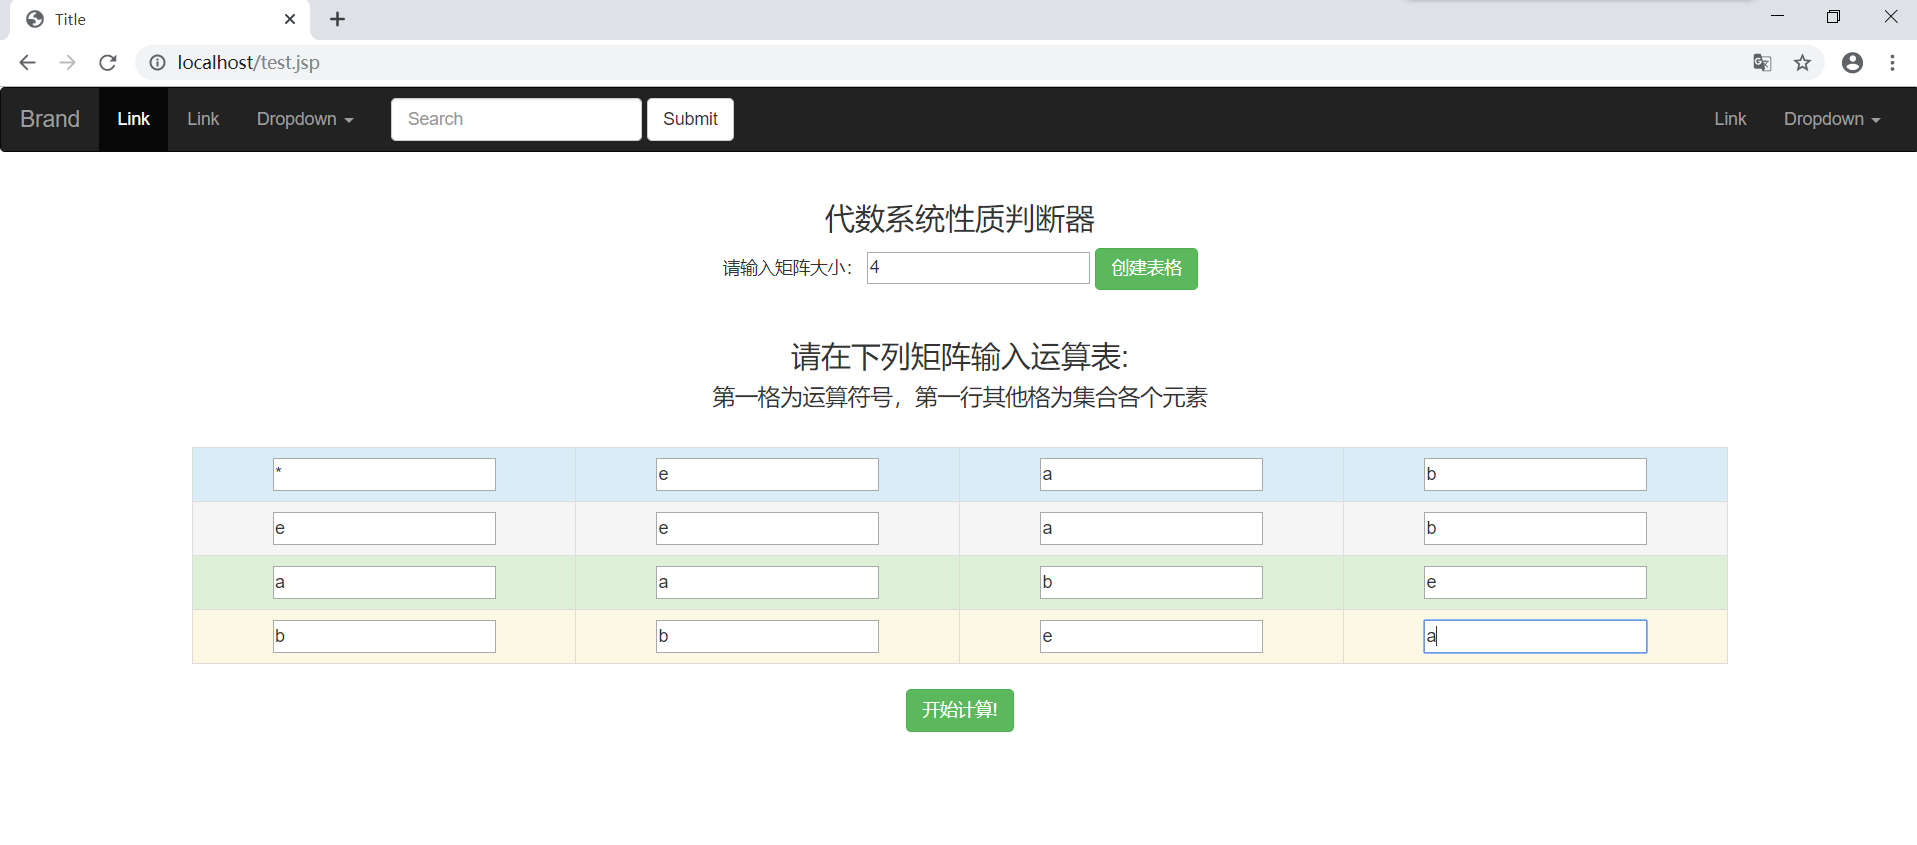
\includegraphics[width=14.7cm,height=6.5cm]{1.png}
    \caption{前端显示图片}
\end{figure}
\begin{figure}
    \centering
    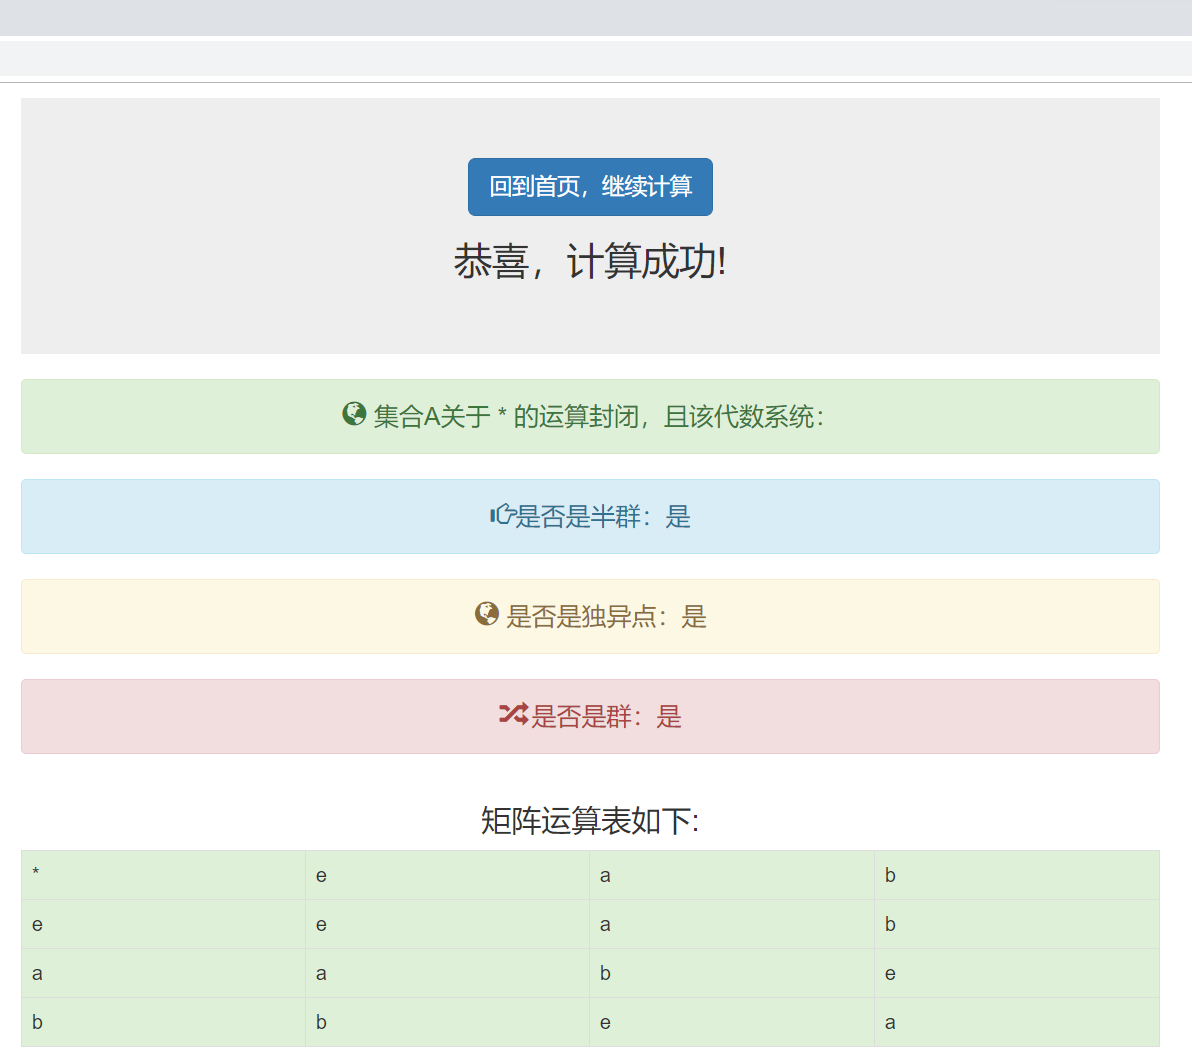
\includegraphics[width=9cm,height=8cm]{2.png}
    \caption{前端显示图片}
\end{figure}
\section{算法核心代码}
\lstinputlisting{Main.Java}
\section{算法核心代码+前端可视化}
\lstinputlisting{Main1.Java}
\end{document}